\documentclass[14pt]{extbook}
\usepackage{multicol, enumerate, enumitem, hyperref, color, soul, setspace, parskip, fancyhdr} %General Packages
\usepackage{amssymb, amsthm, amsmath, latexsym, units, mathtools} %Math Packages
\everymath{\displaystyle} %All math in Display Style
% Packages with additional options
\usepackage[headsep=0.5cm,headheight=12pt, left=1 in,right= 1 in,top= 1 in,bottom= 1 in]{geometry}
\usepackage[usenames,dvipsnames]{xcolor}
\usepackage{dashrule}  % Package to use the command below to create lines between items
\newcommand{\litem}[1]{\item#1\hspace*{-1cm}\rule{\textwidth}{0.4pt}}
\pagestyle{fancy}
\lhead{Progress Quiz 1}
\chead{}
\rhead{Version B}
\lfoot{4082-7053}
\cfoot{}
\rfoot{test}
\begin{document}

\begin{enumerate}
\litem{
Write the equation of the line in the graph below in Standard form $Ax+By=C$. Then, choose the intervals that contain $A, B, \text{ and } C$.
\begin{center}
    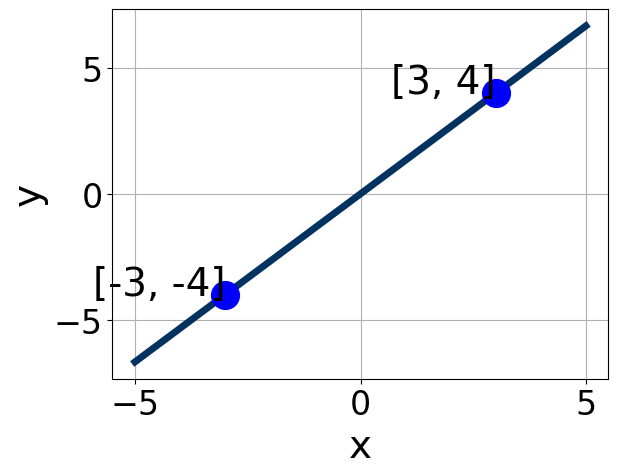
\includegraphics[width=0.5\textwidth]{../Figures/linearGraphToStandardB.png}
\end{center}
\begin{enumerate}[label=\Alph*.]
\item \( A \in [0.13, 1.63], \hspace{3mm} B \in [-3.6, 0.2], \text{ and } \hspace{3mm} C \in [-2, 5] \)
\item \( A \in [1.51, 3.33], \hspace{3mm} B \in [3.2, 6.2], \text{ and } \hspace{3mm} C \in [-2, 5] \)
\item \( A \in [0.13, 1.63], \hspace{3mm} B \in [-0.9, 4.6], \text{ and } \hspace{3mm} C \in [-2, 5] \)
\item \( A \in [-3.4, -0.18], \hspace{3mm} B \in [-5.2, -4.6], \text{ and } \hspace{3mm} C \in [-2, 5] \)
\item \( A \in [1.51, 3.33], \hspace{3mm} B \in [-5.2, -4.6], \text{ and } \hspace{3mm} C \in [-2, 5] \)

\end{enumerate} }
\litem{
Find the equation of the line described below. Write the linear equation as $ y=mx+b $ and choose the intervals that contain $m$ and $b$.\[ \text{Parallel to } 5 x + 6 y = 10 \text{ and passing through the point } (6, -4). \]\begin{enumerate}[label=\Alph*.]
\item \( m \in [-0.95, -0.15] \hspace*{3mm} b \in [-11.6, -9.6] \)
\item \( m \in [-1.94, -1.04] \hspace*{3mm} b \in [-0.9, 2] \)
\item \( m \in [-0.95, -0.15] \hspace*{3mm} b \in [-0.9, 2] \)
\item \( m \in [-0.95, -0.15] \hspace*{3mm} b \in [-1.7, 0.2] \)
\item \( m \in [0.54, 1.39] \hspace*{3mm} b \in [-9.4, -7.9] \)

\end{enumerate} }
\litem{
Solve the equation below. Then, choose the interval that contains the solution.\[ -4(-5x -3) = -18(6x + 12) \]\begin{enumerate}[label=\Alph*.]
\item \( x \in [1.49, 1.94] \)
\item \( x \in [-1.78, -1.56] \)
\item \( x \in [-2.06, -1.69] \)
\item \( x \in [-2.38, -2.2] \)
\item \( \text{There are no real solutions.} \)

\end{enumerate} }
\litem{
Find the equation of the line described below. Write the linear equation as $ y=mx+b $ and choose the intervals that contain $m$ and $b$.\[ \text{Perpendicular to } 4 x + 5 y = 14 \text{ and passing through the point } (-5, -5). \]\begin{enumerate}[label=\Alph*.]
\item \( m \in [-2.1, 0.04] \hspace*{3mm} b \in [-11.88, -10.82] \)
\item \( m \in [0.68, 1.08] \hspace*{3mm} b \in [1.1, 1.34] \)
\item \( m \in [1.15, 1.88] \hspace*{3mm} b \in [-1.71, -1.06] \)
\item \( m \in [1.15, 1.88] \hspace*{3mm} b \in [1.1, 1.34] \)
\item \( m \in [1.15, 1.88] \hspace*{3mm} b \in [-0.29, 0.74] \)

\end{enumerate} }
\litem{
Write the equation of the line in the graph below in Standard form $Ax+By=C$. Then, choose the intervals that contain $A, B, \text{ and } C$.
\begin{center}
    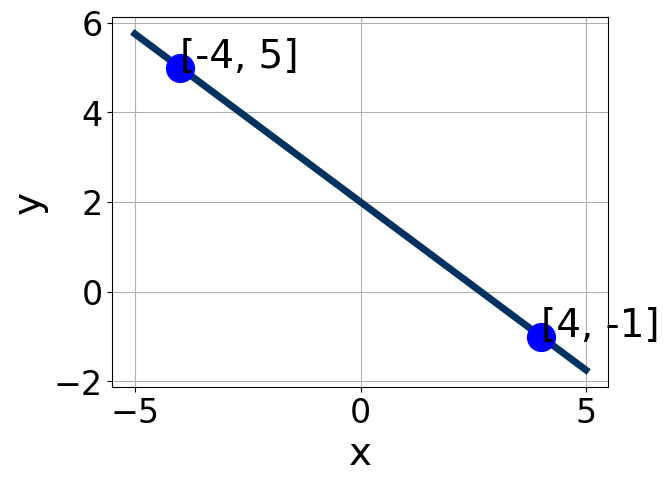
\includegraphics[width=0.5\textwidth]{../Figures/linearGraphToStandardCopyB.png}
\end{center}
\begin{enumerate}[label=\Alph*.]
\item \( A \in [1, 11], \hspace{3mm} B \in [-7.5, -3.5], \text{ and } \hspace{3mm} C \in [22, 28] \)
\item \( A \in [-0.4, 2.6], \hspace{3mm} B \in [-4.7, 0.4], \text{ and } \hspace{3mm} C \in [0, 7] \)
\item \( A \in [1, 11], \hspace{3mm} B \in [2.2, 7], \text{ and } \hspace{3mm} C \in [-26, -21] \)
\item \( A \in [-0.4, 2.6], \hspace{3mm} B \in [0, 1.4], \text{ and } \hspace{3mm} C \in [-7, 4] \)
\item \( A \in [-5, 0], \hspace{3mm} B \in [-7.5, -3.5], \text{ and } \hspace{3mm} C \in [22, 28] \)

\end{enumerate} }
\litem{
Solve the linear equation below. Then, choose the interval that contains the solution.\[ \frac{-3x -5}{7} - \frac{-3x -9}{2} = \frac{8x -7}{4} \]\begin{enumerate}[label=\Alph*.]
\item \( x \in [10.85, 13.85] \)
\item \( x \in [0.69, 2.69] \)
\item \( x \in [-4.73, -2.73] \)
\item \( x \in [4.96, 7.96] \)
\item \( \text{There are no real solutions.} \)

\end{enumerate} }
\litem{
Solve the equation below. Then, choose the interval that contains the solution.\[ -6(-17x + 19) = -11(7x + 16) \]\begin{enumerate}[label=\Alph*.]
\item \( x \in [-3, -1.4] \)
\item \( x \in [11.4, 13.8] \)
\item \( x \in [-1.2, 0.6] \)
\item \( x \in [-0.2, 2.3] \)
\item \( \text{There are no real solutions.} \)

\end{enumerate} }
\litem{
First, find the equation of the line containing the two points below. Then, write the equation as $ y=mx+b $ and choose the intervals that contain $m$ and $b$.\[ (2, 3) \text{ and } (10, 5) \]\begin{enumerate}[label=\Alph*.]
\item \( m \in [-0.04, 0.77] \hspace*{3mm} b \in [-3.17, -1.43] \)
\item \( m \in [-0.04, 0.77] \hspace*{3mm} b \in [-6.63, -4.17] \)
\item \( m \in [-0.04, 0.77] \hspace*{3mm} b \in [2.27, 2.65] \)
\item \( m \in [-0.61, -0.12] \hspace*{3mm} b \in [5.96, 7.78] \)
\item \( m \in [-0.04, 0.77] \hspace*{3mm} b \in [-0.25, 2.15] \)

\end{enumerate} }
\litem{
Solve the linear equation below. Then, choose the interval that contains the solution.\[ \frac{-3x -7}{5} - \frac{4x -7}{6} = \frac{-9x -9}{4} \]\begin{enumerate}[label=\Alph*.]
\item \( x \in [-2.46, -1.69] \)
\item \( x \in [-9.71, -9.02] \)
\item \( x \in [-0.13, 0.7] \)
\item \( x \in [-1.22, -0.78] \)
\item \( \text{There are no real solutions.} \)

\end{enumerate} }
\litem{
First, find the equation of the line containing the two points below. Then, write the equation as $ y=mx+b $ and choose the intervals that contain $m$ and $b$.\[ (5, -5) \text{ and } (-10, 8) \]\begin{enumerate}[label=\Alph*.]
\item \( m \in [0.6, 4.6] \hspace*{3mm} b \in [16.3, 17.2] \)
\item \( m \in [-1.3, -0.8] \hspace*{3mm} b \in [-2.2, 0.1] \)
\item \( m \in [-1.3, -0.8] \hspace*{3mm} b \in [-11.2, -8.6] \)
\item \( m \in [-1.3, -0.8] \hspace*{3mm} b \in [17.6, 19] \)
\item \( m \in [-1.3, -0.8] \hspace*{3mm} b \in [0.3, 2.2] \)

\end{enumerate} }
\end{enumerate}

\end{document}